% called by main.tex
%
\chapter{Scope}
\label{ch::chapter4}

\section{Hypothesis}

The purpose of this section is to set out in detail, and concisely both the scope of this project, and the main objectives that have been pursued. It seeks to collect new information as from the time of doing this study, there weren’t any others that used the techniques mentioned in the previous section to classified audios and advancing the field of HIE detection among neonates. The results from this study will be made easier to extrapolate, and be applied to other projects that are currently developing different solutions within this same line of research. This holistic approach allows for a more comprehensive understanding of the possible practical application and implementation of the project in other settings for better HIE diagnosis. 


\begin{tcolorbox}
This project is divided into two phases, the first phase tests different models (\textbf{MLP}, \textbf{SVM}, \textbf{LSTM}) with a public dataset optimising the parameters until satisfactory results are obtained. Then in the second phase, the models are adjusted, and trained with real data (HUBU dataset) from this project.
\end{tcolorbox}

\section{Main objective}
Apart from the objectives that have been mentioned in the Objectives (Section \ref{ch::chapter2}), it is essential to clarify, and detail in depth, the specific purpose of this project, and how its results can be applied in real contexts. 


\begin{tcolorbox}
In this context, the specific objective of the project is to develop a dataset with arrays that detect crying in every second of the recorded audio. This way of presenting the results is crucial, as it provides an essential tool that can later be integrated with other datasets generated by parallel projects. 
\end{tcolorbox}

These projects analyse different aspects of how the neonate reacts to a stimulus, focusing on visual elements, and combined with the results from this study ultimately generates a multidisciplinary approach that increases the understanding of the responses that the neonate may make for improved HIE detection.

\section{Interrelation with other projects}
In the scheme presented in the image \ref{fig:general-project} you can see the integration of the projects that are currently being developed within the \myurl{https://gicap.ubu.es/main/home.shtml}{Applied High Performance Computing Research Group (GICAP)} of the University of Burgos, for the detection of HIE. Within this multidisciplinary group, each research line covers specific areas related to the neonatal response to different stimuli. These areas include, the identification of spasms, and arm or leg movements, as well as the detection of whether the mouth or eyes remain open or closed, and the classification of facial expressions such as frowning, and other visual cues. 

The findings from these responses are intended to provide an understanding, and classification of the infant's state of alertness. This understanding is crucial to critically intervene in a timely manner if abnormalities in the newborn's behaviour are detected.
\newline
\begin{figure}[h]
\centering
    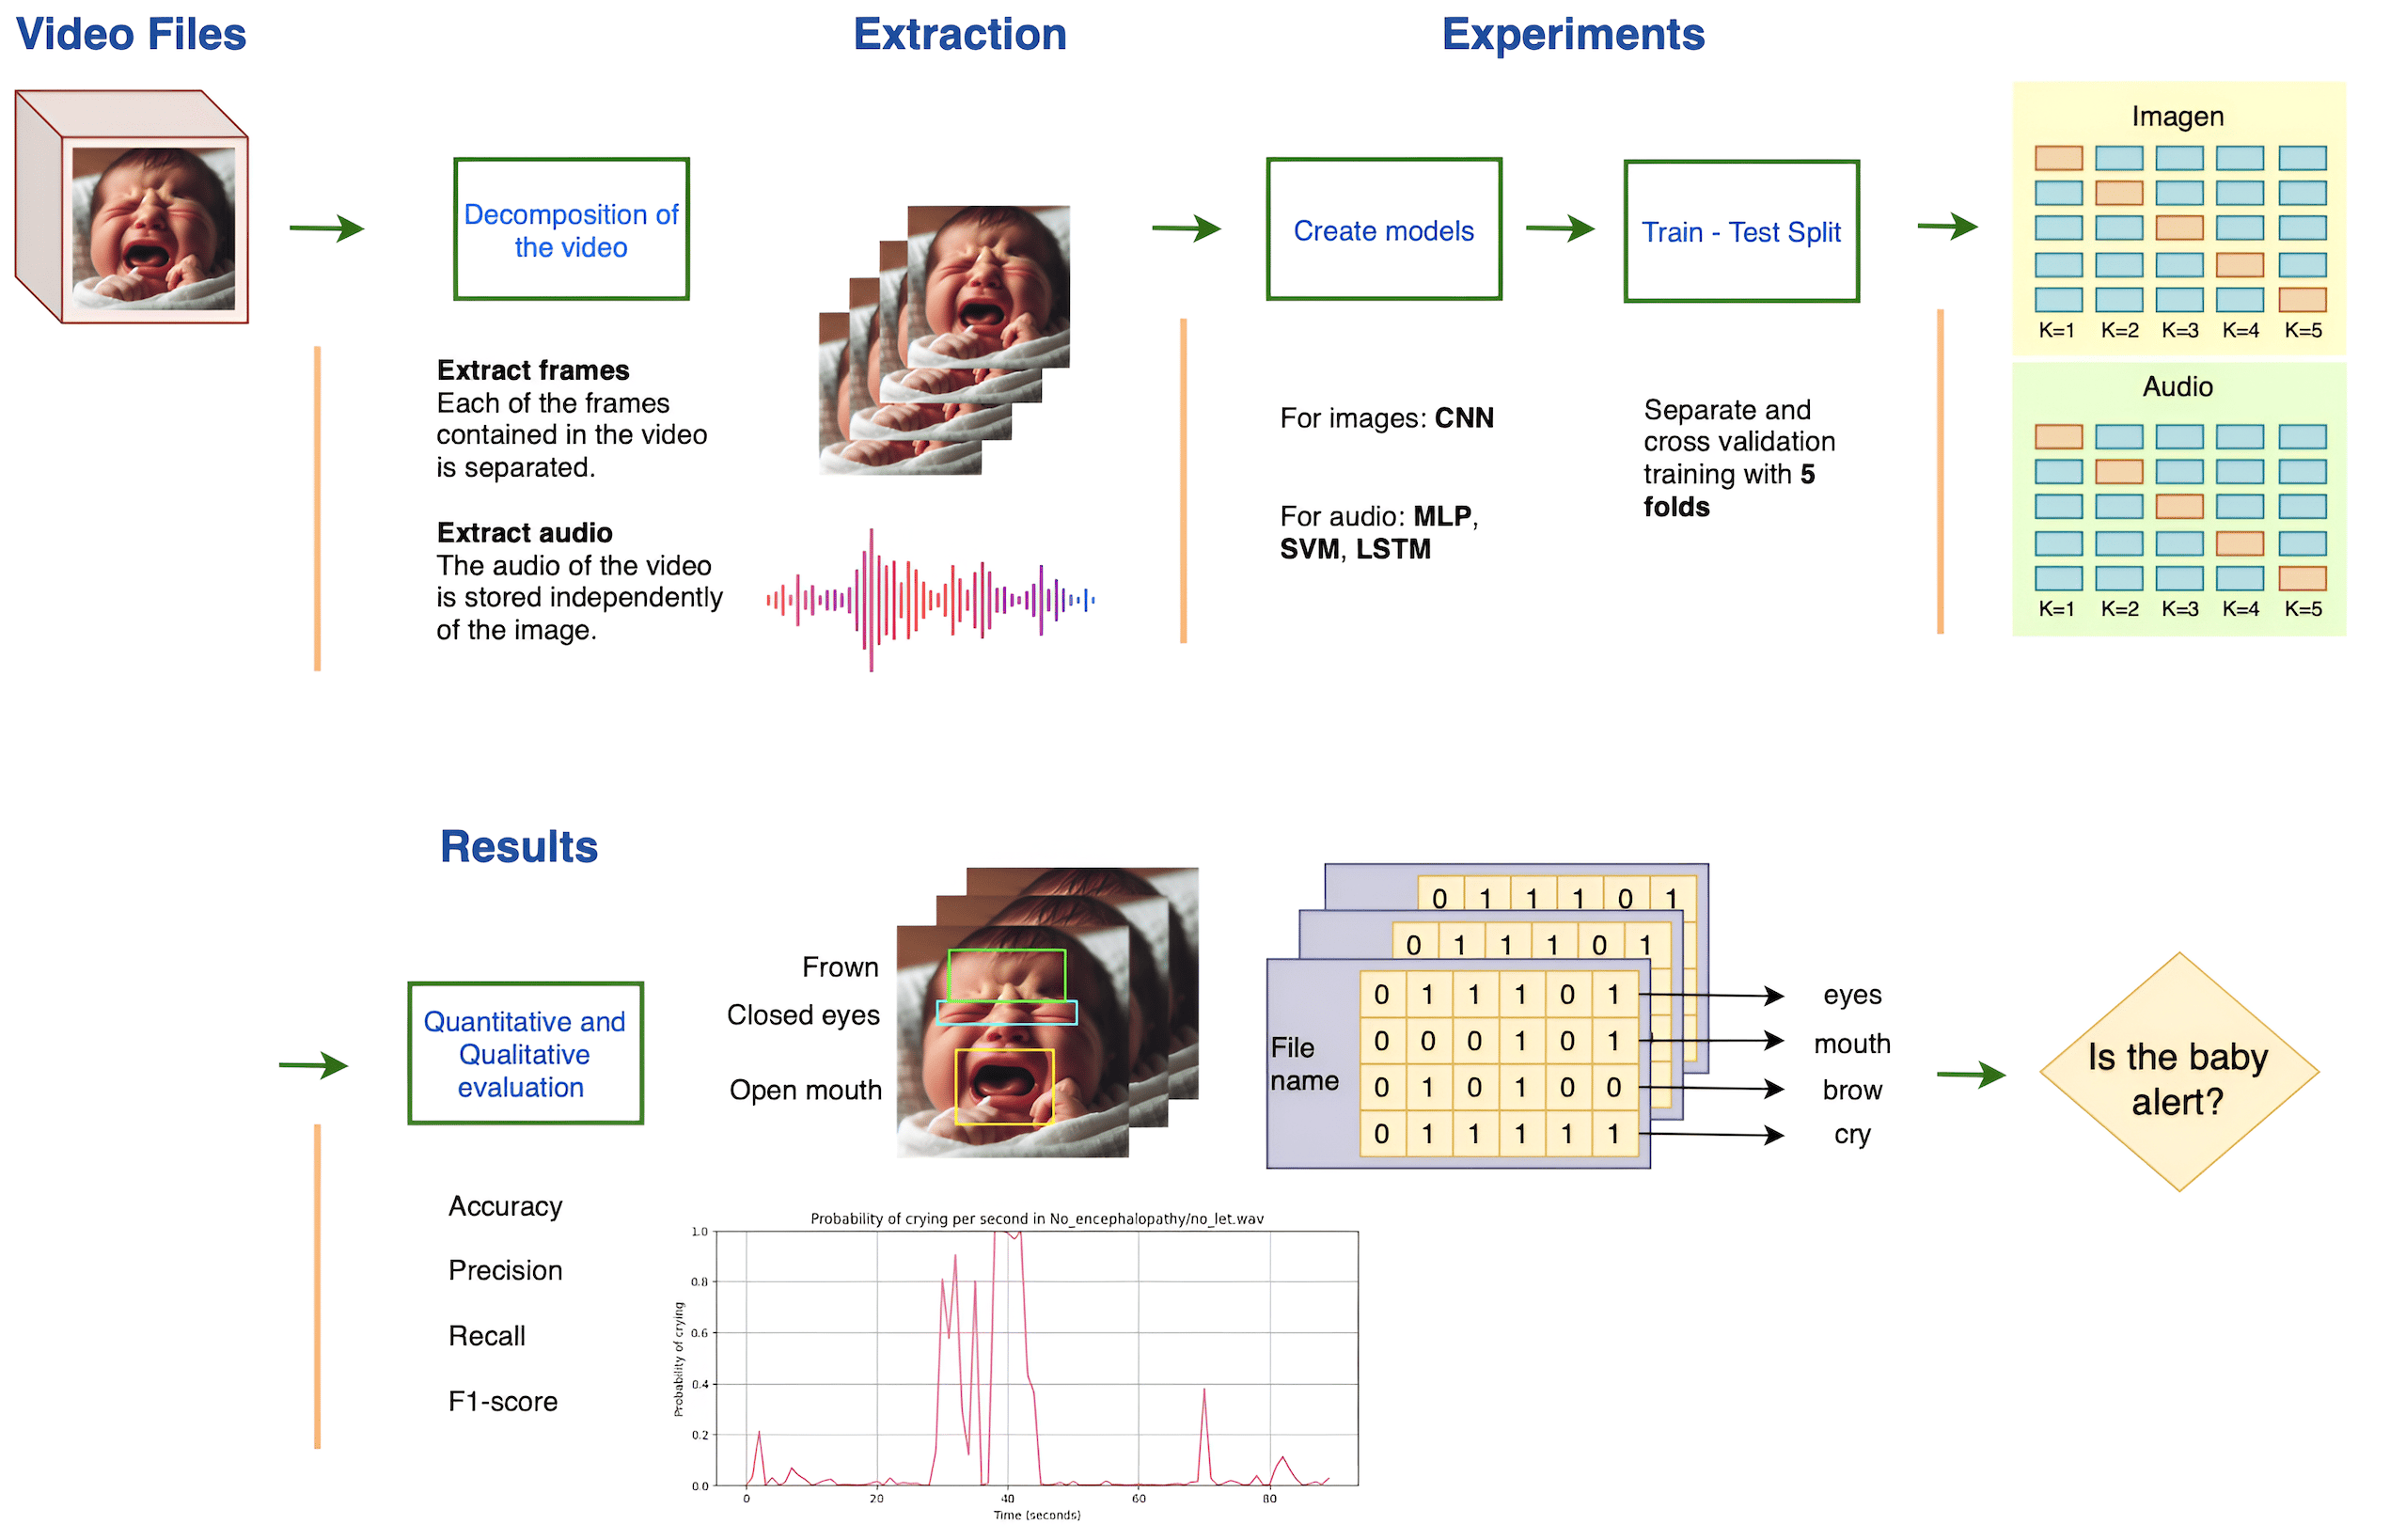
\includegraphics[width=1\textwidth]{figures/General-project.png}
\caption{Pipeline of the project interrelated with other projects}
\label{fig:general-project}
\end{figure}

\section{First steps}
The first steps consisted of a thorough evaluation to determine whether the CNN techniques used in the classification of images of neonates’ facial expressions for HIE detection in the work by mentioned in the previous section, could be utilized for sound classification in this study for the same purpose. This preliminary approach is essential to understand the overall development of the project and to establish a correct methodological approach that can be transferred and applied to the field of audio classification. 

Initially, the possibility of continuing with the line of work (Convolutional Neural Networks (CNN) to classify the images of neonates’ facial expressions) by GICAP group was raised. In this study, with audios of neonates, the acoustic signal was transformed into a waveform representation, which allowed visualising the intensity of the sound over time. Once this representation was created, it was hypothesised that the peaks with the highest amplitude corresponded to the moments when the baby was crying.

\begin{figure}[h]
\centering
    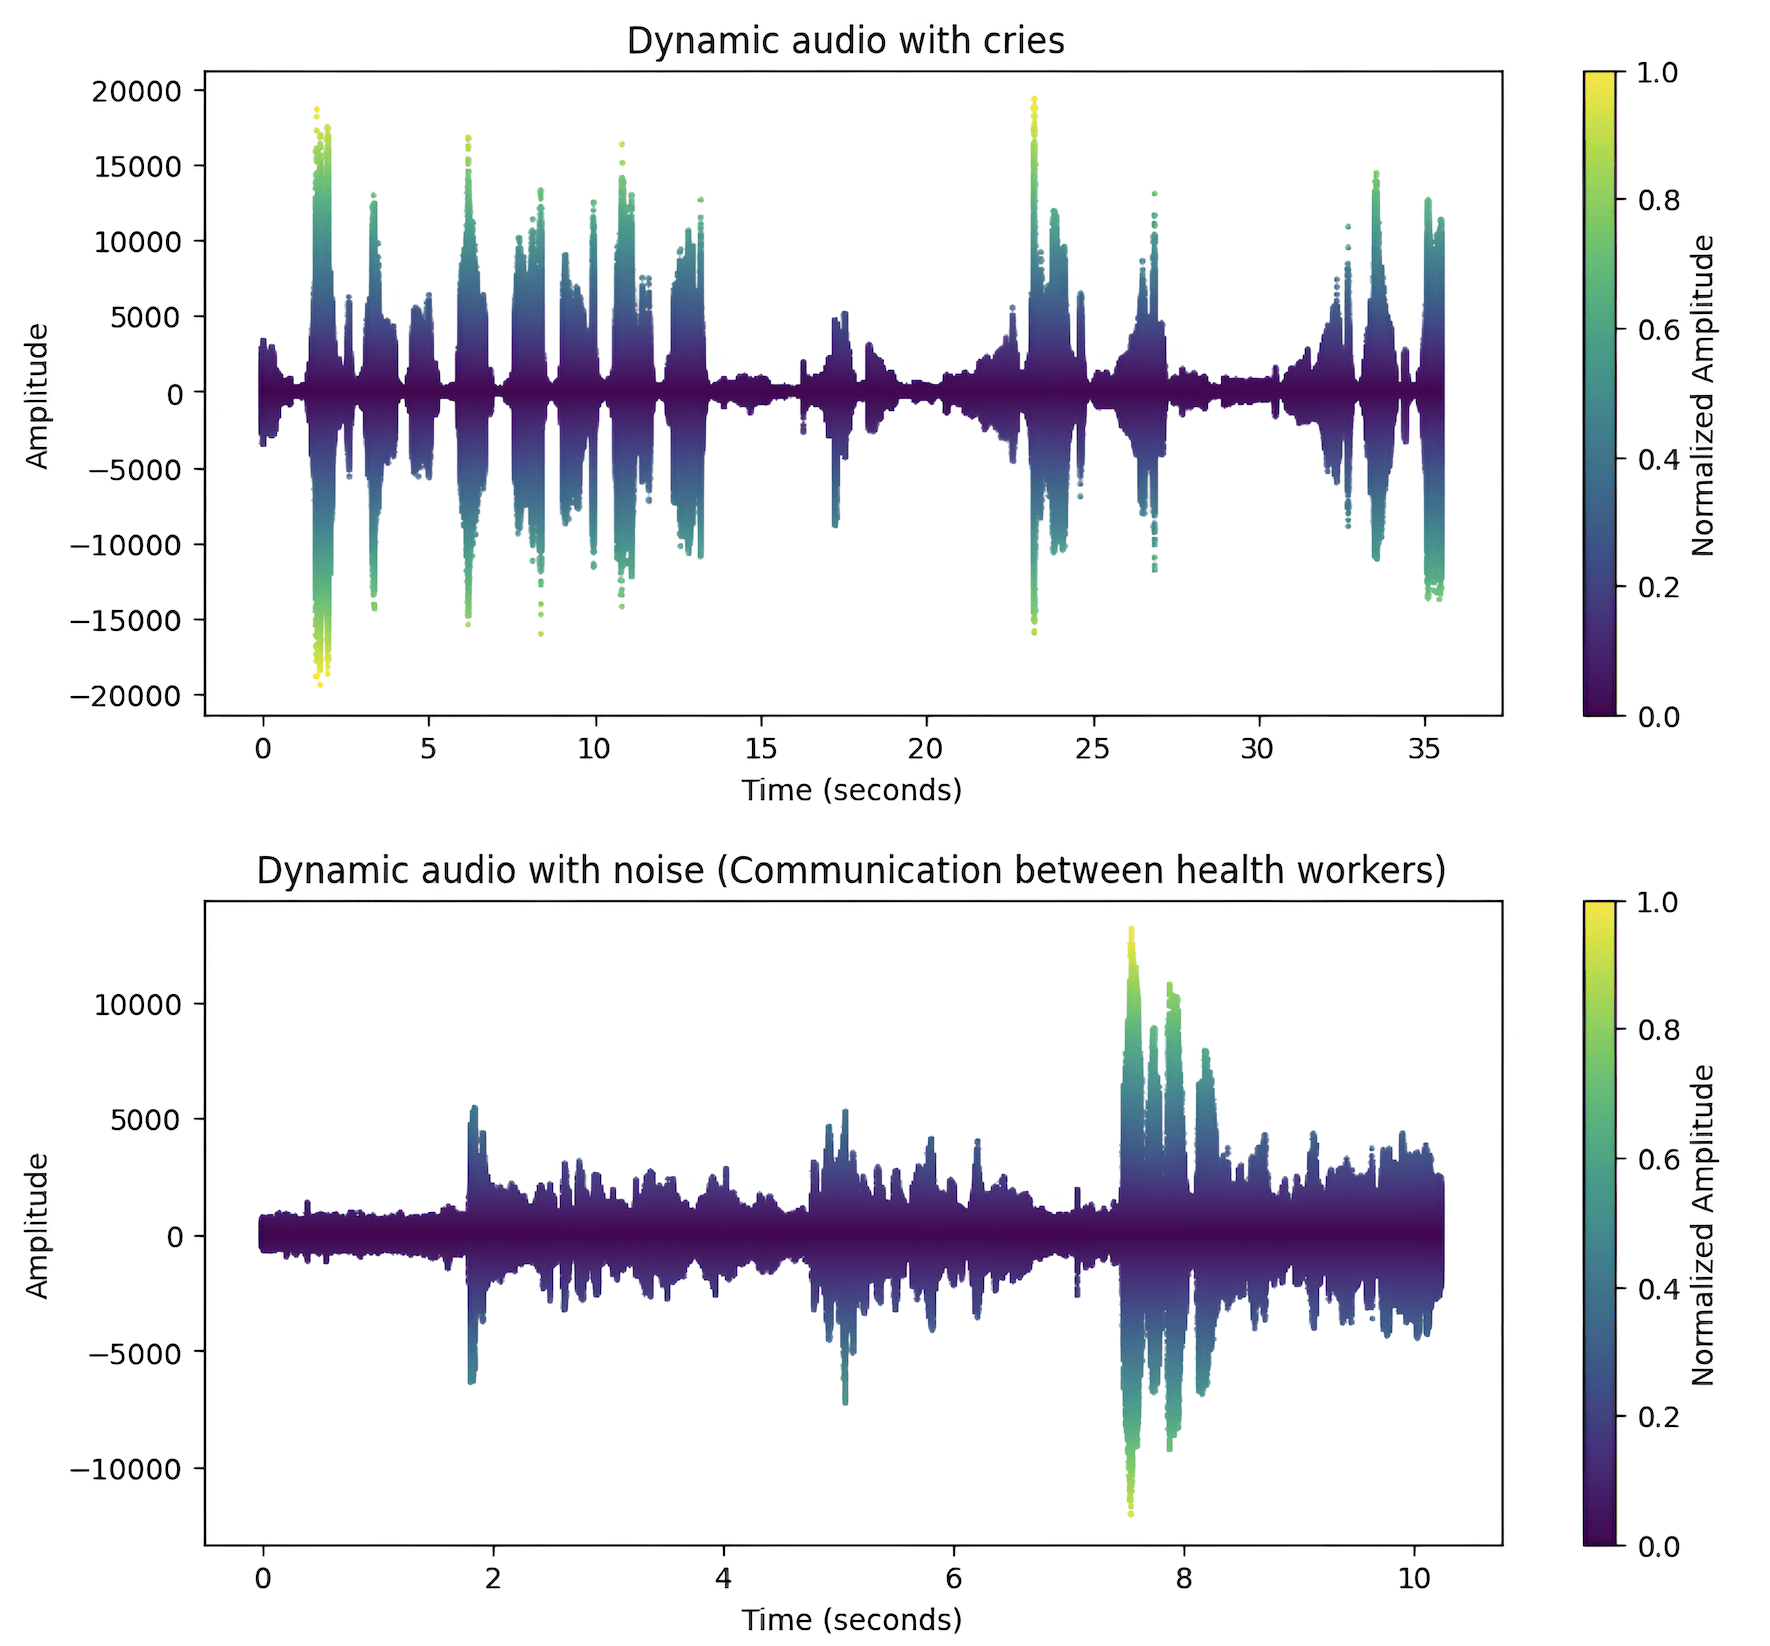
\includegraphics[width=0.5\textwidth]{figures/waveform.png}
\caption{Waveform of different audio files}
\label{fig:waveform}
\end{figure}

The above technique, the Python \textbf{PyDub} library has been used, which is responsible for loading and processing the stored audio files. \textbf{Parallel to the audio representation process, a process of analysis of the different sounds in the audios in each available file was followed}. These audios contain a variety of sounds, including, the main sounds expected to be heard, which are the cries of the neonates, but also instructions, and communications among healthcare personnel, or noises from different medical devices can also be heard. This means that the times when the waveforms reach a higher amplitude do not always correspond to a baby's cry. This issue can be clearly seen in the waveform comparisons in the image \ref{fig:waveform}. In the first waveform, the baby's cry predominates, making the image a viable, and a good alternative to select the moments when the amplitude peaks in order to identify the cry. However, the second waveform represents an audio in which there is no baby crying but includes other types of sounds. In this second scenario, the limitations of using waveforms for baby cries’ detection are evident, as they only identify different types of sound according to their intensity.


This gap presents the need to develop a more sophisticated approach for audio classification. The main goal of this project is to effectively classify neonatal cries, regardless of the intensity with which the neonate cries, or the variety of sound sources with which it is mixed. This is crucial because the audios researchers work with are from babies who are only a few hours old or who have delicate health conditions. For this reason, on many occasions, acoustic reactions to stimuli are expected which may be minimal, and just a slight whimper could be decisive in determining the baby's state of health.

\section{Second steps}
After discarding the first line of action, and addressing the limitations that were found, a review of scientific articles \cite{Bashiri2020, Chang2020, Ji2020, K2021, Liang2022, zabidi2009classification, Wahid2016, Orlandi2016} focused on finding solutions to problems similar to the one faced by this project. With this review, a new approach to the project was generated that focused on the possibility of implementing dissimilar machine learning models. In this case, a group of widely recognised models for audio classification were selected: Multi-Layer Perceptron (\textbf{MLP}), Support Vector Machines (\textbf{SVM}), and Short-Term Memory Neural Networks (\textbf{LSTM}). Different Python libraries have been used for the development of these models, in particular the \textbf{Scikit-learn} library to integrate the MLP, and SVM models, and \textbf{TensorFlow} plus \textbf{Keras} to develop the LSTM model.

Once the implementation of machine learning models was chosen, the first drawback arose: \textbf{the videos available for audio classification (HUBU videos) were not labelled}, which created a problem in the supervised training of the selected models. These models depend on input examples with real labels so that later, during training, they learn from the input data, and finally make the predictions in the test phase. 

To resolve this drawback, a \textbf{public dataset} was used to test the selected models. This dataset is organised in a directory structure as shown in the image \ref{fig:public-dataset}. Each directory contains 108 short audio files classified according to the type of sound each one stores.

With this labelled dataset, feature extraction was carried out using various techniques, which are discussed in more detail below. Several experiments have been carried out, some with and some without five-fold cross-validation to assess the generalisation of the models. This was checked using test data, and performance metrics such as \textbf{accuracy}, \textbf{F1-score}, \textbf{precision}, and \textbf{recall} that resulted in satisfactory performance for each of the models, that have been used with the real data of this project.
